\subsection{Other Experiments}
To further explore the classification problem, we conducted additional experiments 
involving CNN-based feature extraction, data augmentation, and a novel approach 
using a tiered ensemble model.

\subsubsection*{CNN-Based Experiments}

We conducted a series of experiments using Convolutional Neural Networks (CNNs) to explore their 
effectiveness as feature extractors for the 5-class classification problem. The CNN was
used with ImageNet weights and was not fine-tuned.

\begin{itemize}[leftmargin=*]
    \item \textbf{VGG16 with Spectral Features}: VGG16 CNN was employed as a feature extractor with 
    spectral features (MFCC, CQT, Chroma STFT, among others) used as input images. This approach yielded 
    a Macro F1 score of approximately 65\%, which is lower than the performance achieved in the primary 
    work.
    \item \textbf{VGG16 with Raw Waveform Images}: VGG16 was also used to extract features from raw 
    waveform images. Features were taken from the 5th, 4th, and 3rd convolutional layers after pooling, 
    and various classifiers (RF, SVM, MLP) were tested on these features. This method resulted in a 
    performance of around 67\%.
\end{itemize}

\subsubsection*{Data Augmentation}
\label{sec:data_augmentation}

We explored data augmentation techniques to address the limited and imbalanced dataset and improve
the model's generalization capabilities.

\begin{itemize}[leftmargin=*]
    \item \textbf{Noise Addition and Speed/Pitch Alteration}: We augmented the data by adding random noise (factor 0.05)
    and altering speed and pitch. However, the improvement in performance was not significant. 
    This may be due to the limited size and inherent imbalance of the dataset, as data augmentation 
    did not alter the class distribution.
    \item \textbf{Synthetic Data Generation with SMOTEN}: Synthetic data generation was applied to the 
    less represented classes using SMOTEN. Although there was an initial spike in performance metrics, 
    this was identified as bias. The model could easily distinguish the synthetically generated data from 
    the original data. The underlying issue was the limited size of the original dataset, which did not 
    provide sufficient variability for the synthetic generation algorithm to produce realistic 
    and diverse samples.
\end{itemize}

\subsubsection*{Tiered Ensemble Model}

We attempted to decompose the classification problem into two sub-problems, according to Figure \ref{fig:tiered_ensemble}.

\begin{itemize}[leftmargin=*]
    \item \textbf{Sub-problem 1: Artifact, Normal, and Abnormal Classification}: Various models were 
    tested for distinguishing between artifact, normal, and abnormal audio. The best model 
    (MLP\_Ensemble5) achieved a balanced accuracy of approximately 89.2\%.
    \item \textbf{Sub-problem 2: Disease Classification}: Different models were also applied to 
    distinguish between different diseases, achieving a balanced accuracy of more than 90.3\% with MLP\_Ensemble2.
    \item \textbf{Final Ensemble Model}: A third model (CatBoost) was used to integrate the predictions 
    from the above sub-problems and make the final classification among the five classes. This ensemble 
    approach resulted in a balanced accuracy of 80.5\%.
\end{itemize}

\begin{figure}[H]
    \centering
    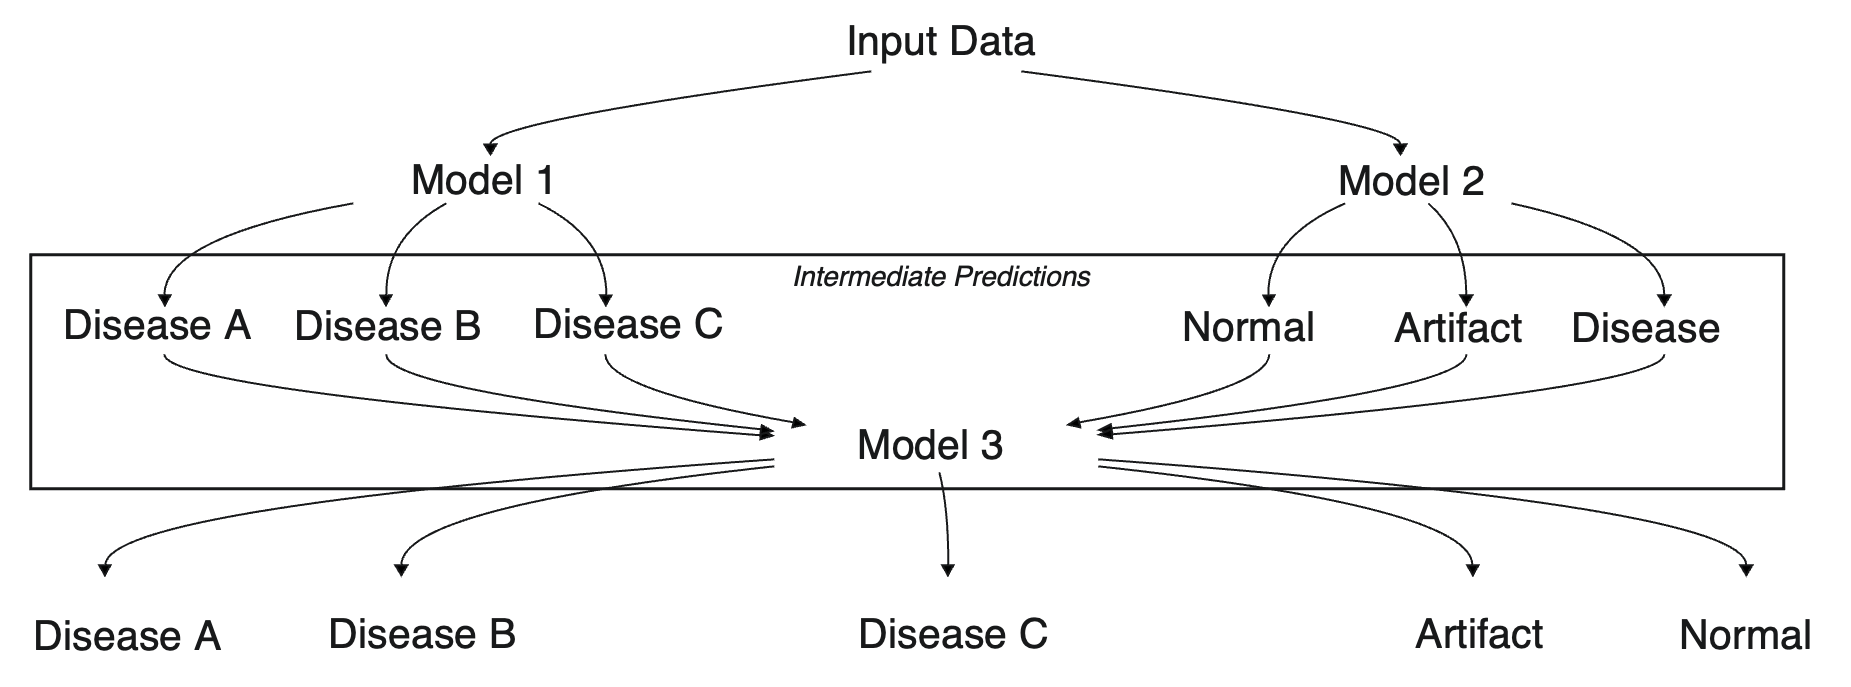
\includegraphics[width=1\columnwidth]{images/tiered_ensemble.png}
    \caption{Tiered Ensemble Model}
    \label{fig:tiered_ensemble}
\end{figure}

\noindent
Despite the promising results, the tiered ensemble model did not outperform the primary models.
